\chapter{Configuración del Vocabulario}

El vocabulario no viene enteramente configurado en ATLAS Broadsea sino tan solo una pequeña demo adjunta a la base de datos de Eunomia, tal y como se describe en el repositorio de github de la \href{https://github.com/OHDSI/Broadsea-Atlasdb/tree/main}{ Base de datos de Broadsea}.

Por tanto, para poder utilizar ATLAS en profundidad se requiere la instalación y configuración del Vocabulario más extenso. OHDSI propone, en el repositorio de github de \href{https://github.com/OHDSI/Broadsea}{Broadsea} dos formas de configurar el vocabulario de Broadsea: (1) de forma manual (2) a través de Apache Solr. 

\section{Configuración manual}

La configuración manual del vocabulario requiere descargrar el vocabulario directamente desde ATHENA, instalarlo manualmente en el directorio local de Broadsea y ejecutar el contenedor docker encargado de montar el vocabulario en Broadsea. 


\subsection{Requisitos previos}

Para configurar el vocabulario manualmente,  se debe haber descargado el vocabulario y configurado el directorio local de Broadsea. Este procedimiento se ha seguido gracias a los foros \href{https://forums.ohdsi.org/t/downloading-omop-cdm-version-5-vocabulary-data/3321/3}{Downloading OMOP cdm version 5 vocabulary data} y \href{https://forums.ohdsi.org/t/march-to-the-broadsea/20576}{March to the Broadsea} y el tutorial de yotutube \href{https://www.youtube.com/watch?v=FCHxAQOBptE}{Demo: Getting Vocabularies Into My OMOP CDM}.

\begin{enumerate}

    \item Descargar el vocabulario desde la herramienta online de  \href{https://athena.ohdsi.org/}{ATHENA}.Para ello, acceder al menú de descarga \code{Download}. En este momento se presenta un listado de todos los vocabularios que contiene ATHENA entre los que algunos aparecen preseleccionados. Cada usuario puede seleccionar o deseleccionar los vocabularios que le interesen para el estudio que esté realizando. En este caso, se descargará el vocabulario que ATHENA sugiere por defecto.
    
    \begin{figure}[H]
        \centering
        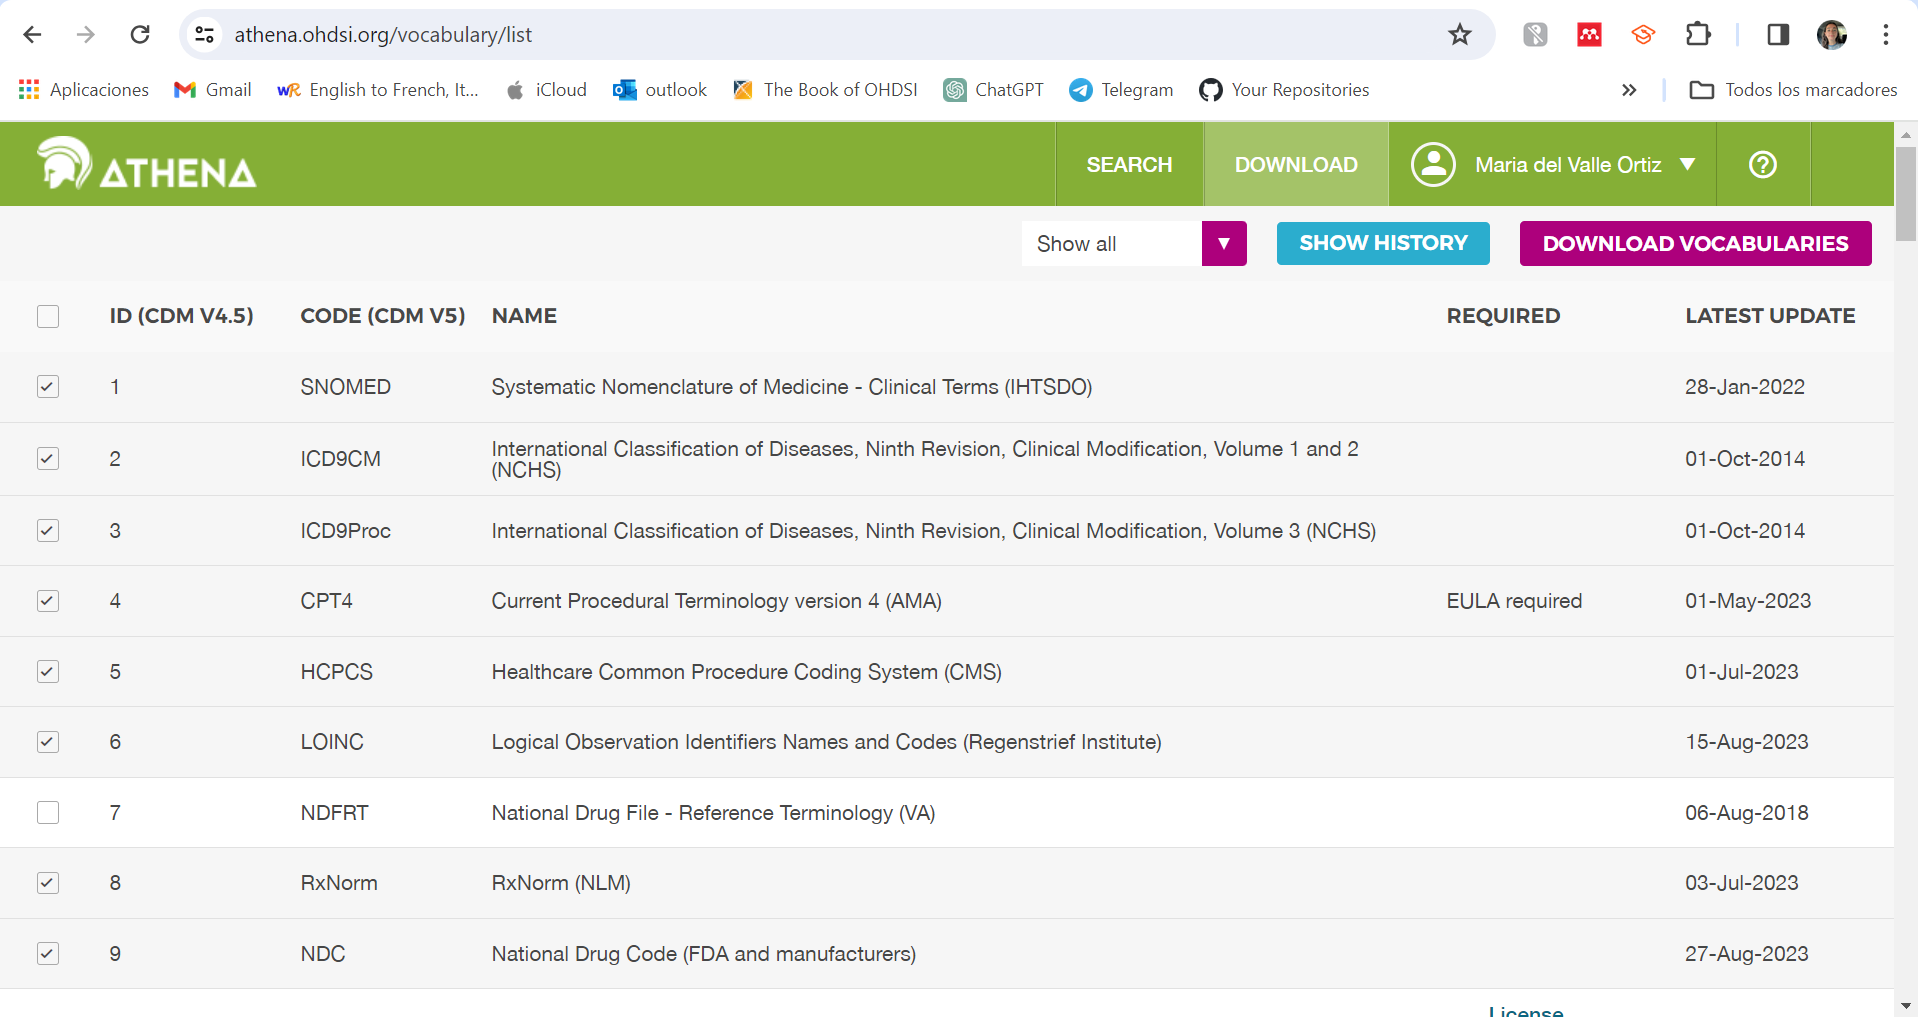
\includegraphics[width=0.90\textwidth]{figures/athenaPreDownload.png}
        \caption{Captura de pantalla de la preselección de vocabularios para descargar.}
        \label{fig:athenaPreDownload}
    \end{figure}

    \item La descarga requiere registrar un usuario con un correo electrónico válido al que se enviará un link personal que permitirá la descarga de un archivo .zip con el vocabulario seleccionado. También desde ATHENA en la pestaña \code{SHOW HISTORY} muestra el estado en el que se encuentra la descarga del vocabulario y, una vez que esté listo, permite la descarga directa del zip.

    \item El archivo zip que se descarga, una vez descomprimido, muestra varios archivos .csv con las tablas que conforman el Vocabulario y otros archivos \textcolor{red}{CPT4 que no serán de interés}. 

      \begin{figure}[H]
        \centering
        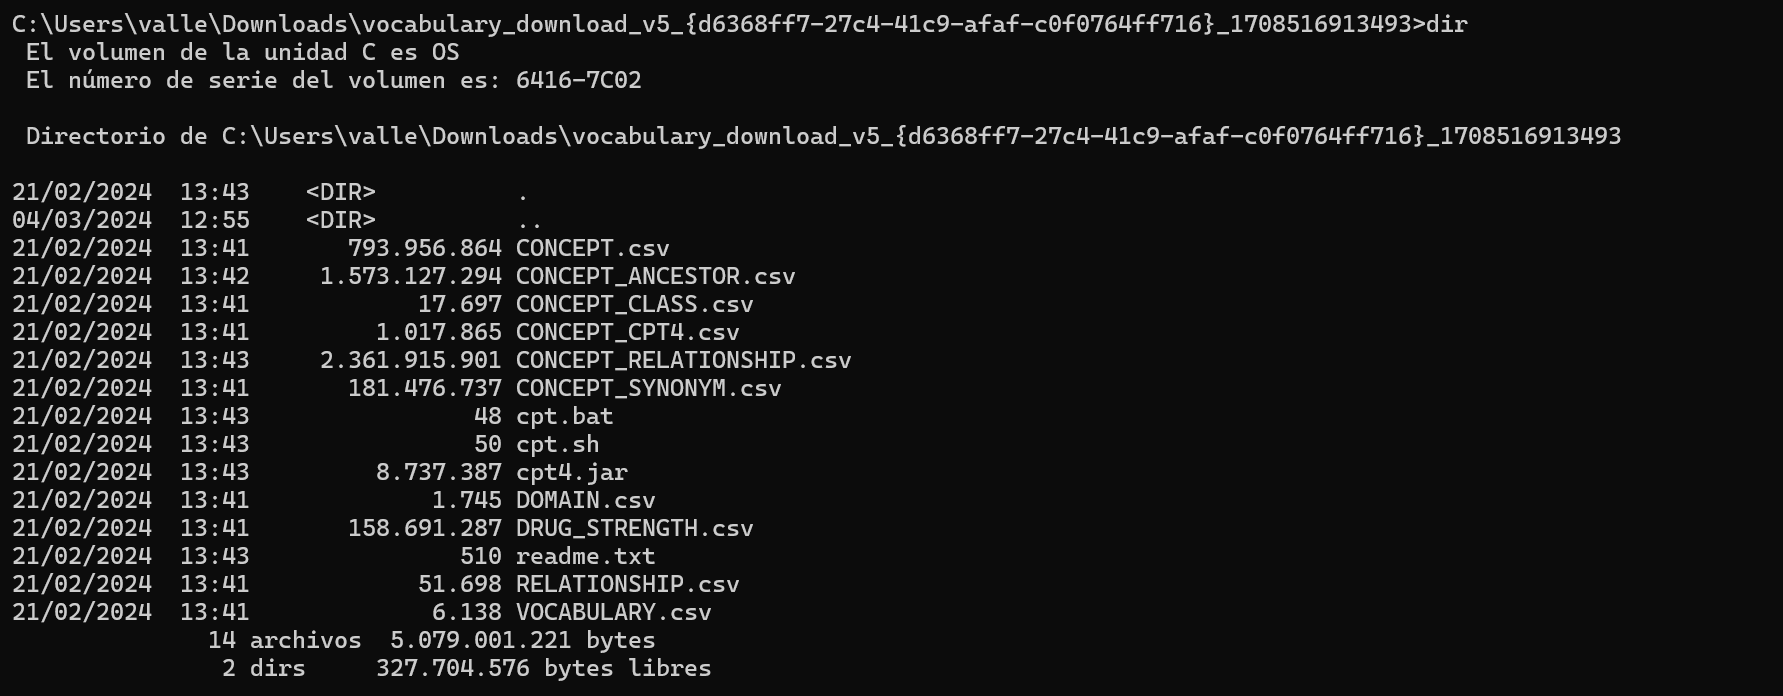
\includegraphics[width=0.90\textwidth]{figures/vocabDownload.png}
        \caption{Captura de pantalla de archivos descargados del vocabulario.}
        \label{fig:vocabDownload}
    \end{figure}

    \item Por último, los archivos descargados del vocabulario deben almacenarse en el directorio local de Broadsea, concretamente en la ruta \code{Broadsea/omop\_vocab/files}. En caso de no existir la carpeta \code{/files}, crearla manualmente. Este paso es muy importante.

\end{enumerate}

\subsection{Deployment}

Configurar el vocabulario requiere establecer una configuración avanzada del contenedor Docker de Broadsea. Si bien, la primera vez que se inicializó el contenedor se ejecutó el perfil \code{default} ahora se va a ejecutar específicamente el perfil \code{omop-vocab-pg-load}. Esta opción se especifica en la sección \href{https://github.com/OHDSI/Broadsea?tab=readme-ov-file#omop-vocab-loading}{OMOP Vocab Loading} del repositorio de Broadsea. También ha sido de utilidad el repositorio \href{https://github.com/OHDSI/WebAPI/wiki/CDM-Configuration}{CDM Configuration} y el mismo forum \href{https://forums.ohdsi.org/t/march-to-the-broadsea/20576}{March to the Broadsea}.

Para acceder a la información y configuración avanzada del perfil se puede acceder al \code{docker-compose.yml} y a la sección 9 del archivo \code{.env}, aunque este caso no será necesario realizar ninguna modificación sobre los mismos.

\begin{enumerate}

    \item Para comenzar la configuración del vocabulario es necesario inicializar el contenedor \code{omop-vocab-load}. Ejecutar la siguiente línea de código en el \code{cmd}:

    \begin{lstlisting}[language=sh]
    docker compose --profile omop-vocab-pg-load up -d\end{lstlisting}

    Este comando da lugar el siguiente resultado.

      \begin{figure}[H]
        \centering
        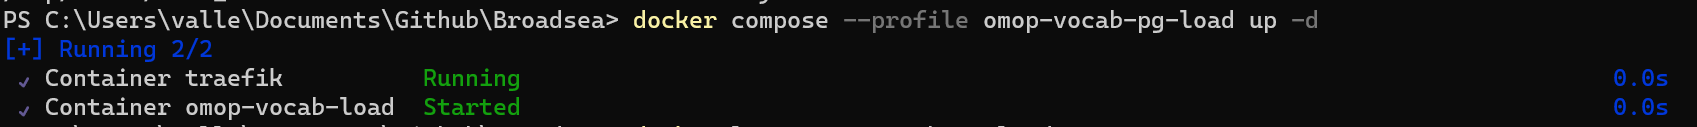
\includegraphics[width=0.90\textwidth]{figures/composeProfVocabLoad.png}
        \caption{Captura de pantalla de comando para iniciar el perfil docker.}
        \label{fig:composeProfVocabLoad}
    \end{figure}

    \item A partir de este momento comienza la instalación del perfil, por lo que es muy importante tener abierto el \code{logs} de Docker para poder observar que el proceso se realiza correctamente. El proceso puede durar unas horas y una vez que se finaliza, el log muestra un mensaje que advierte que el contenedor puede ser eliminado y el estado del contenedor pasa a ser ''Exited''. El resultado es la creación de un nuevo esquema en la base de datos llamado ''omop\_vocab'' con todos los archivos descargados del vocabulario. 

    \item El último paso de la configuración es integrar este nuevo esquema a la WebAPI de Broadsea. Este último paso se puede realizar fácilmente de forma manual a través de pgAdmin, abriendo la tabla \code{source\_daimon} del esquema \code{webapi} de la bd de Broadsea.

    La instalación por defecto de Broadsea adjudica la fuente del vocabulario (\code{daimon\_type=1}) al \code{demo\_cdm}, sin embargo, se debe modificar para que apunte al nuevo esquema \code{omop\_vocab} que se ha instalado. Esta modificación se puede realizar directamente sobre la tabla que devuelve la siguiente consulta.

    \begin{lstlisting}[language=sql]
    SELECT * FROM webapi.source_daimon
    ORDER BY source_daimon_id ASC \end{lstlisting}

    El resultado debe ser similar a la siguiente figura.

    \begin{figure}[H]
        \centering
        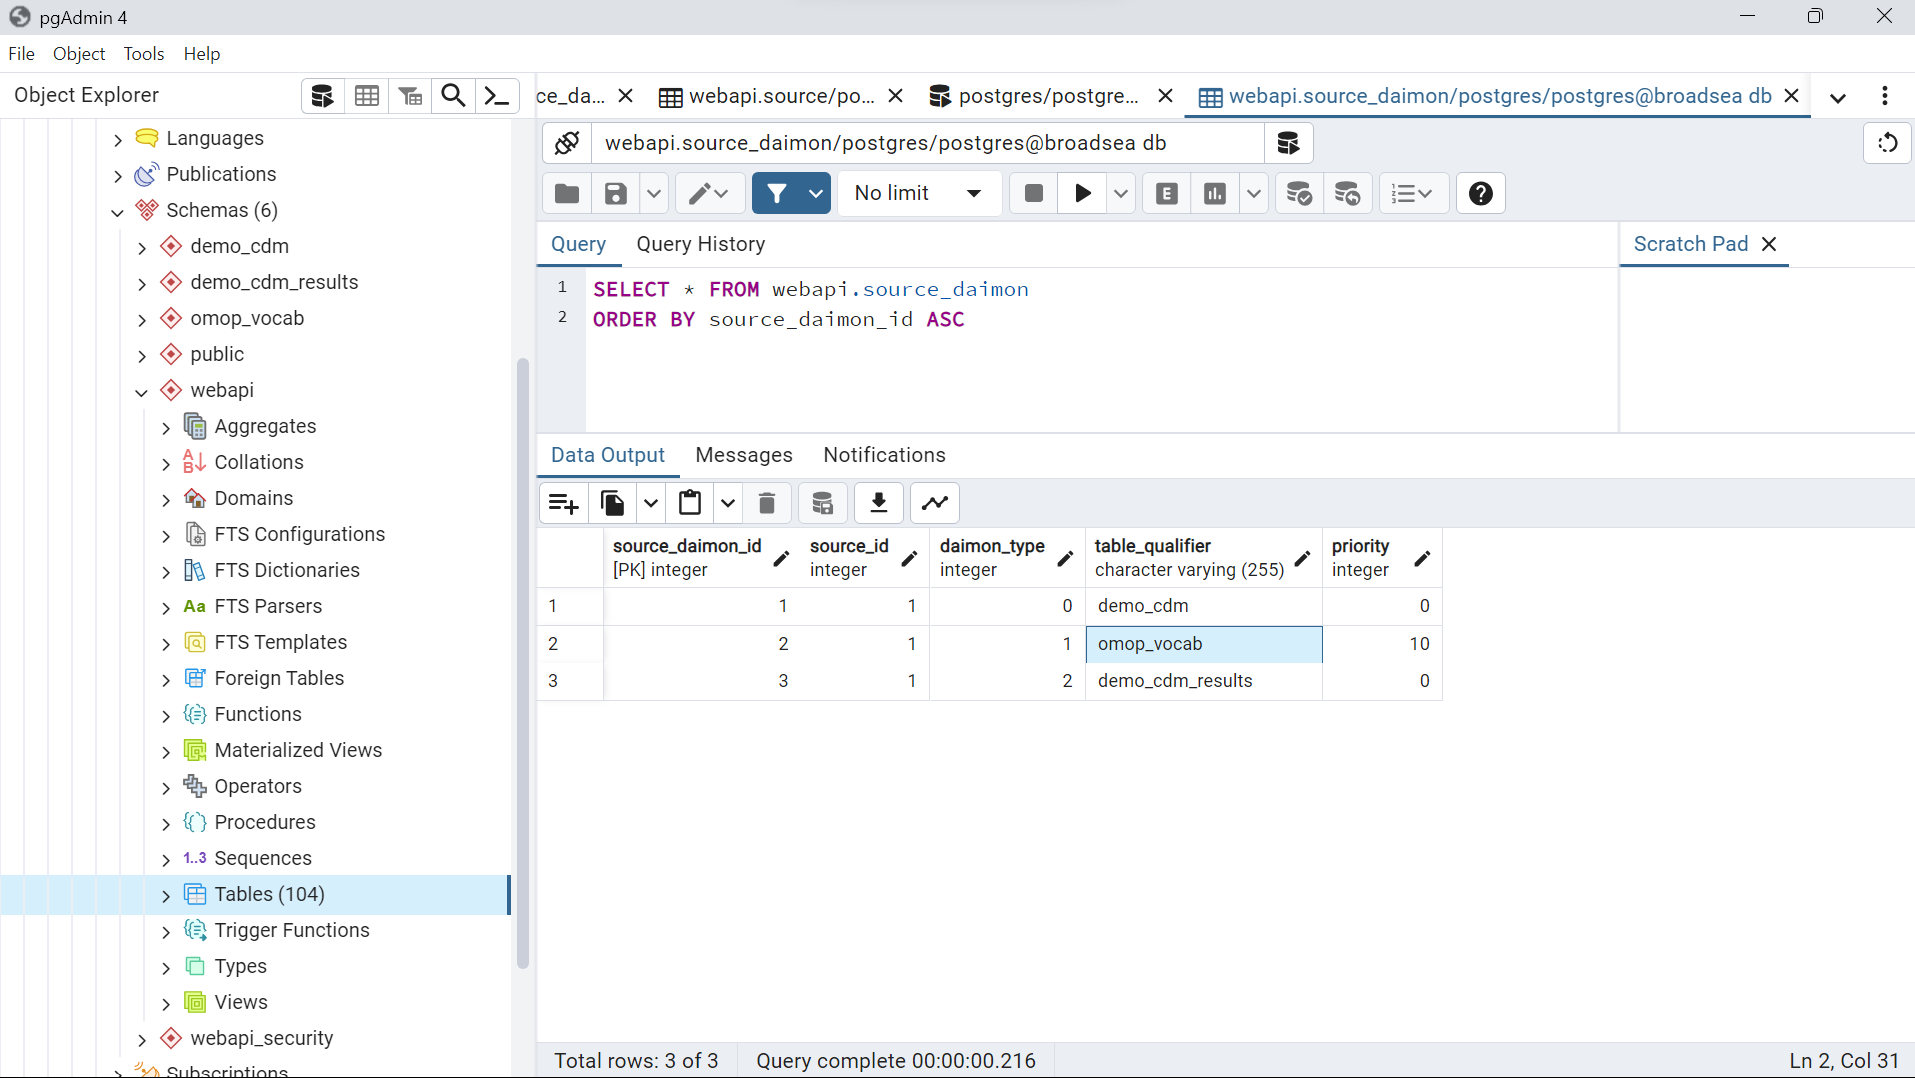
\includegraphics[width=0.90\textwidth]{figures/omopVocabResult.png}
        \caption{Captura de pantalla de la integración final del vocabulario descargado con la webapi}
        \label{fig:omopVocabResult}
    \end{figure}

\end{enumerate}

\subsection{Comprobación de configuración correcta}

Para comprobar que se ha configurado correctamente el vocabulario en la base de datos de Broadsea, se puede (a) consultar el administrador de la base de datos y (b) realizar una búsqueda en ATLAS.

- comprobar que se ha instalado correctamente y no vacío en pgADmin

- comprobar que se ha relacionado con broadsea mediante atlas


\begin{enumerate}

    \item La comprobación consultando el administrador de la base de datos implica abrir pgAdmin, acceder al servidor y a la base de datos de Broadsea y revisar el listado de esquemas. Debe aparecer un nuevo esquema denominado \code{omop\_vocab}.
    
    A continuación, para comprobar que el esquema se haya instalado completamente, se puede seleccionar cualquiera de las tablas que lo componen, click derecho \code{View data/All rows} y comprobar que la tabla no esté vacía. En este ejemplo se ha utilizado la tabla \code{vocabulary} para realizar la comprobación.

 \begin{figure}[H]
        \centering
        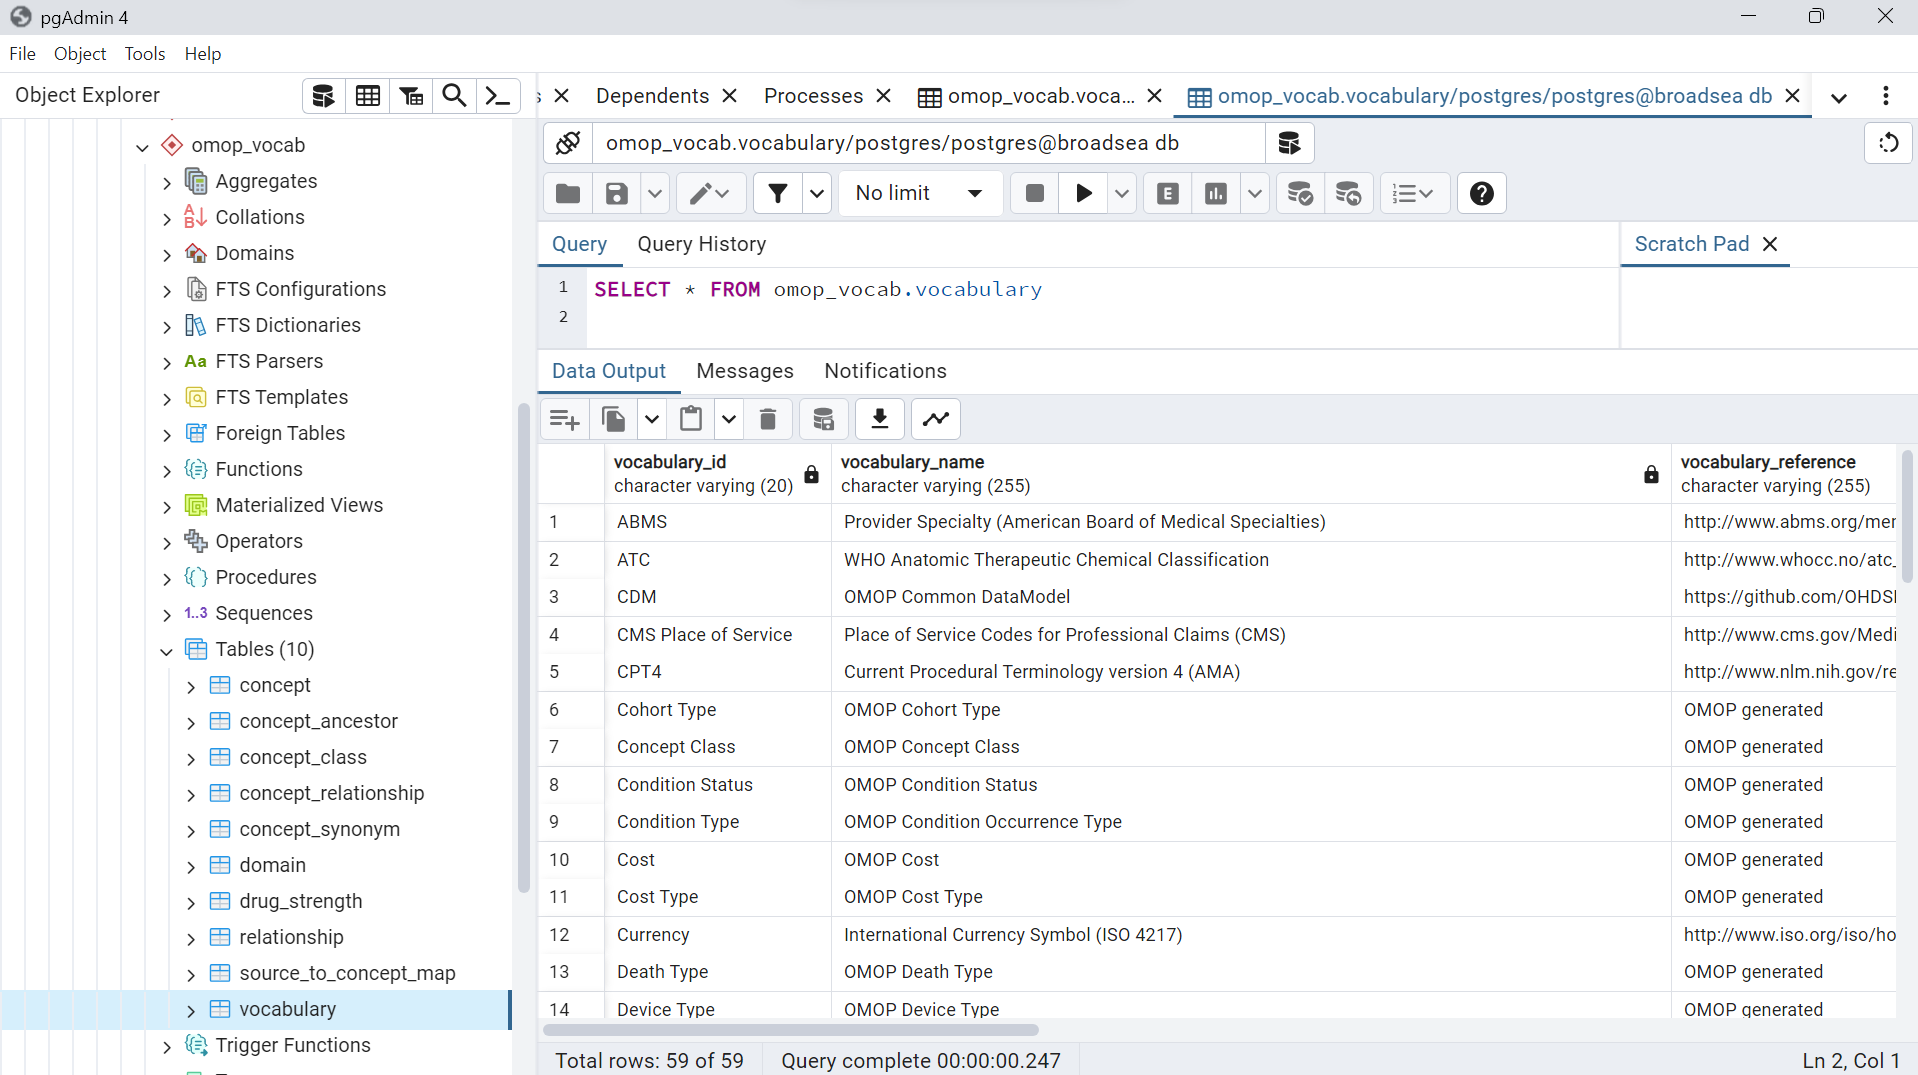
\includegraphics[width=0.90\textwidth]{figures/omopVocabComprobacion.png}
        \caption{Captura de pantalla de comprobación de configuración correcta del vocabulario en pgAdmin.}
        \label{fig:omopVocabComprobacion}
\end{figure}

    \item Otra opción es realizar un búsqueda en ATLAS
    
\end{enumerate}

\subsection{Solución de posibles errores}

- No haber creado la carpeta /files

- Haber creado la carpeta /files pero vacía

- Se crea el esquema pero se queda vacío: ESPERATE A QUE SE EJECUTE EL CONTENDOR 

\section{Configuración mediante Apache Solr}

- Indexador de la BD. No procede pero se presenta.

- Se ha intentado. No se ha podido.. Está bajo desarrollo aún.

- Issue en github y forum.

\section{Configuración de PHOEBE}

- Recomendador de conceptos del vocabulario. No procede pero se presenta.

